% main.tex, to be used with thesis.tex
% This contains the main work of your thesis.

%\bibliography{thesis}  % uses the references stored in Chapter1Radar.bib

\chapter{Data Persistence for Sensor Networks: A Case Study for NetBEAMS}
\label{chap:netbeams-overview}

As discussed in Chapter 2, different properties of a sensor network and the
nature of the collected data must be taken into account in order to provide a
data persistence layer for a given sensor network. Similarly, in order to
better assist one's analysis of such functionality, Chapter 3 proposed a set of
data persistence taxonomies related to different properties of the collected
data life cycle. The goal of this chapter is to describe the fundamental properties 
of the case study used for this work, that is, NetBEAMS, in order to lay the 
groundwork as it relates to the selection of the database technology. NetBEAMS 
provides an automated infrastructure solution for SF-BEAMS, and this last component 
will be covered first. Then, this work proposes a categorization of NetBEAMS to 
the face of the taxonomies.

\section{SF-BEAMS: a Marine Sensor Network for Water Quality Monitoring}

As described by \cite{netbeams2009}, NetBEAMS is a joint venture between the
department of Biology and Computer Science at San Francisco State University,
whose goal is to automate the operational execution of SF-BEAMS. The San Francisco
Bay Environmental Assessment and Monitoring Station, or SFBEAMS \cite{sfbeams2006}, 
is an environmental sensor network system whose primary focus is the study of complex 
marine and estuarine environments using the SF-BEAMS sensors. The sensors are deployed off a
pier located on the San Francisco Bay, in Tiburon, California; and is operated by 
the Romberg Tiburon Center for Environmental Studies (RTC) a part of San Francisco
State University. NetBEAMS is an experimental component that utilizes the SF-BEAMS 
infrastructure to operate. This section details SF-BEAMS in general, and
presents the requirements for data persistence after classifying NetBEAMS based
on the taxonomies defined in the previous chapter.

\subsection{The SF-BEAMS Infrastructure}
\label{sec:sfbeams}

The SF-BEAMS sensor network is responsible for providing data for water quality
monitoring, as well as weather and surface conditions. Figure
\ref{fig:sf-beams} shows a picture taken from the SF-BEAMS web-camera.

\begin{figure}[!t]
  \centering
    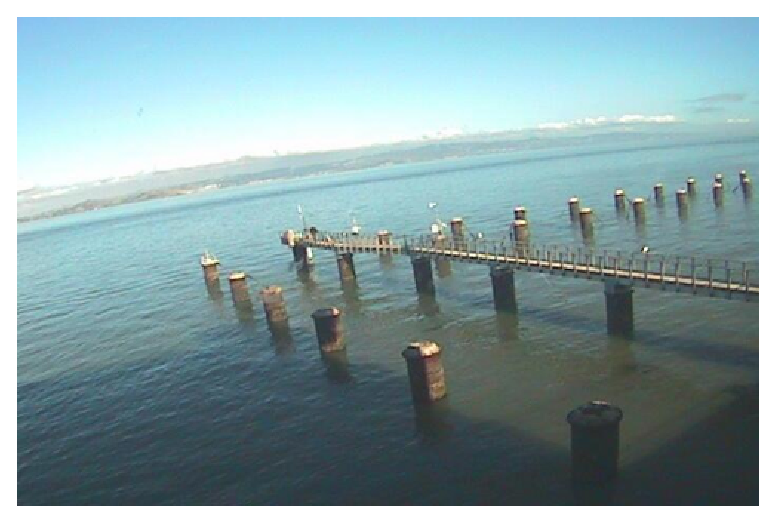
\includegraphics[scale=0.7]{../diagrams/cam_image-oct15}
  \caption{Picture of the SF-BEAMS Network, at the RTC pier. Tiburon, CA.}
  \label{fig:sf-beams}
\end{figure}

In general, the SF-BEAMS network infrastructure contains a varying number of
wired and wireless devices attached to pylons at the pier. Each of them
is responsible for observing different conditions of the area, having its own
mechanisms for internal storage for the collected data. In this way, data can
be directly transferred to the labs via Ethernet cables or collected manually
with a laptop computer. The current data collection process for SF-BEAMS is
described in Figure
\ref{fig:SF-BEAMS-system-architecture}\cite{sfbeams-current-system}. Upon
collecting data from sensors, the RTC staff uses automation scripts written in
Matlab \cite{matlab} to process, index and distribute the raw data in
different formats. One of these formats is the OPeNDAP \cite{opendap}, which
is widely used at research institutions to promote easier data exchange
amongst them. The SF-BEAMS website provides access to the collected data through
the Internet at http://sfbeams.sfsu.edu:8080/opendap. An example of an HTTP
Request from accessing the data for a specific YSI \cite{YSI-Sonde} is shown in
Listing \ref{file:rtc-ysi-opendap}.

\begin{figure}[!b]
  \centering
  \includegraphics[scale=0.5]{../diagrams/SF-BEAMS-system-architecture}
  \caption{The Current SF-BEAMS Data Collection Process}
  \label{fig:SF-BEAMS-system-architecture}
\end{figure}

As described in section \ref{sec:sn-infrastructure}, sensor devices produce
the observed data based on properties of measurements defined by its
manufacturer. NetBEAMS has used ``YSI 6600 ESD V2" \cite{YSI-Sonde}, as seen
in Figure \ref{fig:ysi-device}, one of the sensors devices used by SF-BEAMS.
It is a powerful water quality-monitoring device, capable of producing around
52 bytes on a single real-time data stream reading, as shown on Table
\ref{tab:ysi-data-stream}.

\begin{figure}[!b]
  \centering
  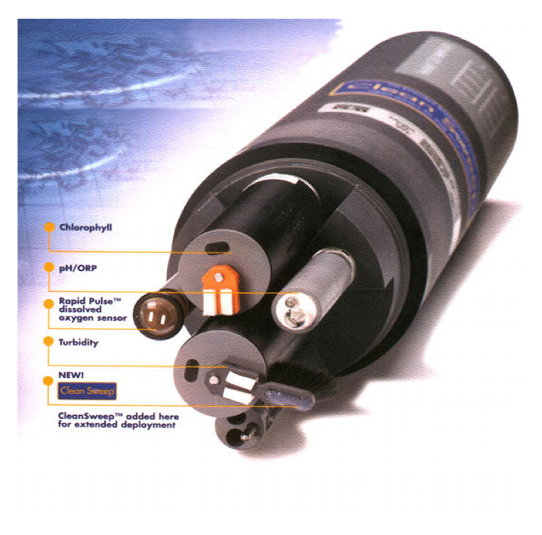
\includegraphics[scale=0.7]{../diagrams/ysi-device}
  \caption{Picture of the case study Sonde device: YSI 6600 ESD V2}
  \label{fig:ysi-device}
\end{figure}

\begin{table}
    \begin{center}
        \begin{tabular}{|l|}\hline
  12.20    192    179 5588.40   0.09   0.084   0.059  7.98   -79.6   99.5  8.83  0.4     8.7\\\hline
        \end{tabular}
    \end{center}
    \label{tab:ysi-data-stream}
    \caption{The Collected Data Stream from the YSI Sonde 6600ESDV2}
\end{table}

In order to have access to the observed data, the network staff downloads the
data using one of the device's connections such as the RS-232 serial connector
\cite{rs232}. Then, they upload the data into their data servers where they are
processed and archived for historical analysis. According to one
staff member, the infrastructure of the SF-BEAMS is comprised of the 
following components (as of May 2009):

\begin{itemize}
  \item 5 YSI Sonde devices, among others, in operation at the RTC pier;
  \item The sampling frequency rate is configured in ranges of either 1, 6 or
  15 minutes, depending on the specification;
  \item The processed data, used for distribution over the Internet,
   contains information regarding the time of the data collection.
\end{itemize}

Considering the infrastructure, the data load in the server-side
of RTC's laboratories produced by the YSI Sonde sensors devices can be
estimated by analyzing the data distribution over a period of one year, as
shown in Table \ref{tab:ysi-data-distribution}:

\begin{table}[!b]
    \label{tab:ysi-data-distribution}
     \begin{center}
      \begin{tabular}{|c|c|c|c|c|c|c|}\hline 
        \textbf{YSIs} & \textbf{Rate} & \textbf{Hourly} & \textbf{Daily} &
        \textbf{Weekly} & \textbf{Monthly} & \textbf{Yearly}\\\hline 
        1 & 1 min & 3.04 Kb & 73.12 Kb & 511.87 Kb & 1.99 Mb & 23.99 Mb\\\hline 
        5 & 6 min & 15.23 Kb & 365.62 Kb & 2.5 Mb & 9.99 Mb & 119.97 Mb\\\hline 
        1 & 15 min & 0.5 Kb & 12.18 Kb & 85.31 Kb & 341.25 Kb & 3.99 Mb\\\hline 
        5 & 1 min & 2.54 Kb & 60.93 Kb & 426.56 Kb & 1.67 Mb & 19.99 Mb\\\hline
        1 & 6 min & 0.2 Kb & 4.87 Kb & 34.12 Kb & 136.5 Kb & 1.6 Mb\\\hline 
        5 & 15 min & 1.0 Kb & 24.37 Kb & 170.62 Kb & 682.5 Kb & 7.99 Mb\\\hline
        \end{tabular}
      \end{center}
    \caption{Amount of data produced by the RTC's YSI sondes}
\end{table}

The maximum amount of data produced by the YSI Sonde device is hundreds of Megabytes
a year, as \textbf{483,840} samples are generated by one single device. 

\subsection{Taxonomic Classification of SF-BEAMS}

This section classifies the sensor network deployed by SF-BEAMS according to
the taxonomies proposed in the previous chapter. This classification is
necessary to better understand the requirements of a data persistence for
NetBEAMS, which indirectly uses the infrastructure of SF-BEAMS.

\begin{itemize}
  \item \textbf{The Purpose of Sensor Data}: the data from SF-BEAMS is exclusively
  used for the purpose of Data Archival, since they are stored in RTC's lab;
  \item \textbf{The Location of the Sensor Data}: it is clear that the purpose
  of the data is directly related to the sensors location and, thus, the
  strategy of \textbf{External Data Storage} is used to store its collected
  data at the network sink at the RTC site;
  \item \textbf{Data Model}: since the format used by the RTC staff to share
  data with researchers is in the OPeNDAP format, the data
  model used is the tabular data model, since it uses the comma-delimited
  files. In this way, the \textbf{Schema-less} model is used;
  \item \textbf{Data Description}: once the collected data reaches the RTC
  lab, a quality assurance process is executed, and the data is transformed
  into the format used by OPeNDAP. This conversion carries data regarding
  the time of the data collection, therefore, one of the
  \textbf{Time Dimensions} such as the valid time is used. Since the files are stored
  with specific file name structure, using timestamps to describe the data, the
  use of transaction time may be also considered. Finally, the contents of the
  files contain the \textbf{Data Identity} as shown in the samples of
  the collected in Listing \ref{file:rtc-ysi-opendap};
  \item \textbf{Query Processing Mechanism}: similar to the data stored in a
  centralized way, the query processing is also \textbf{Centralized}, as the
  data is stored on file system;
  \item \textbf{Data Volume}: the volume of data produced is characterized by small.
 It is related to the volume of data produced by the sensor devices,
  which is numerical data streams, and the total number of sensor devices;
  \item \textbf{System Organization}: SF-BEAMS runs on a Single System, as
  the collected data is stored directly in the file-system after previous 
  processing. However, the collected data is provided to the Internet using
  the OPeNDAP Hyrax system as a middleware.
\end{itemize}

\section{NetBEAMS: a component-based approach for SF-BEAMS}
\label{sec:problem-requirements}

Although the execution of RTC's sensor network can be operated as it
was mentioned in the previous sections, \cite{netbeams2009} described some of the
operational challenges faced by the RTC staff during regular activities of the
data collection process. It was clear to the research group that SF-BEAMS
could have not only its data gathering process automated, but also its data
management and distribution. By the use of COTS\footnote{Common-Off-The-Shelf
designates a product that is produced and sold in bulk} embedded devices and
open-source \cite{open-source} software, the research group developed a second
version of NetBEAMS, a component-based approach which suggested the improvement of 
operational activities from SF-BEAMS using systems automation. In brief, one of the 
ongoing problems of NetBEAMS was regarding Data Persistence, the primary motivation of
this report.

The Networked Bay Environmental Assessment and Monitoring System, or Net-BEAMS,
offers the Data Sensor Platform (DSP) \cite{netbeams2009} as the system
architecture that can address the operation of SF-BEAMS. The in-depth
documentation describing the DSP Platform, including its architecture and data
gathering process is provided at the online documentation 
\cite{netbeams-dsp-architecture}.

The scope of this work is defined as to provide a persistence layer for
NetBEAMS, making a selection of a persistence layer that is an exception to the
taxonomical classification of SF-BEAMS. Furthermore, the technology to be
selected for the persistence layer must take into account the requirements of
NetBEAMS primary users such as Computer Science researchers, as well as end
users such as Biologists from the RTC laboratories. The requirements for the
data persistence specifically for NetBEAMS are described in the following
section.

\section{Requirements for NetBEAMS Data Use}

The main reason for the operation of SF-BEAMS using NetBEAMS's automated
approach is that it can potentially reduce operational costs and improve the
data collection process. In view of this, the scope of a persistence layer
can be summarized as a group of functional and non-functional requirements in
order to select a database system for the sensor network supported by NetBEAMS.

\subsection{Functional Requirements}

\begin{itemize}
  \item Reuse the NetBEAMS infrastructure and develop a component responsible
  for data persistence in a database system;
  \item The Persistence System must obey to the characteristics of the
  categorization of SF-BEAMS used by the taxonomies.
\end{itemize}

\subsection{Non-Functional Requirements}

\begin{itemize}
  \item The data model used to describe the data must not impose restrictions
  to the users of the system (i.e. Biologists and students without expertise in
  Database Systems);
  \item Data Representation must be similar to those used by RTC, with a
  more human-readable format;
  \item The system must be scalable with a low degree of maintenance, in a
  way that the interruptions to the data gathering process are infrequent;
  \item Data must be searchable in near-real-time with good performance;
  \item The system must also support export capabilities, which may
  be used to match RCT's requirements of the OPeNDAP format;
  \item The database must be free of charge, following the
  implementation specifications of NetBEAMS for Open-source software.
\end{itemize}

In conclusion, after detailing the SF-BEAMS sensor network, and describing the 
infrastructure of NetBEAMS, its the motivation and goals for this project were 
presented. The next chapter is the actual analysis of existing database systems 
mentioned in Chapter 2, which aligns with the requirements and characteristics of 
NetBEAMS. Meanwhile, more details regarding the architecture of NetBEAMS, as well as
the development guidelines can be found in the appendix of chapter 10.
